\documentclass[../MaxHughesThesis.tex]{subfiles}

\begin{document}
Due to uncertainties in how to deal with the gamma-beta sum spectrum, the central value of the Fierz term is not ready to be stated. 
However, most of the systematic effects can still be calculated.
The effect with the lower beta cut is likely due to the normalization of the beta-gamma sum spectrum.
The issue is a solvable one. 

\section{Discussion of Results}

The statistical uncertainty of $b_{GT}$ is 0.0042.
This is with 7000000 events that pass the gamma coincidence.
If the lower beta cut uncertainty is excluded, the total systematic uncertainty is 0.0066.
This also excludes any uncertainty on the normalization of the gamma-beta sum spectrum.
This is dominated by the uncertainty of the offset.
If the lower beta cut uncertainty can be resolved, the total systematic uncertainty should only be a touch higher than 0.0066.
This is larger than the statistical uncertainty.
The largest systematic uncertainty is due to the offset, however.
Increasing the number of events should decrease this uncertainty.
The next largest systematic effect is the uncertainty on the $b_{WM}$.
Increasing the number of counts will not decrease the uncertainty of $b_{GT}$ below 0.0028.
A new measurement of $b_{GT}$ would need to be done.

\section{Results Compared to Other Measurements of the Fierz Term}

A similar measurement was done with ultra-cold neutrons \cite{Hic17}.
The beta energy spectrum was measured using a magnetic spectrometer.
The neutrons were confined in the center with a magnetic field, and allowed to decay.
A superratio was used to extract the Fierz term.
With the systematic effects, the final results of the Fierz term was $0.067 \pm 0.005_{stat}$ $ ^{+0.090}_{-0.061} sys$.
Even with the lower beta cut effect, the systematic uncertainty of the Fierz term in the $^{20}$F measurement is much smaller.
The statistical uncertainty is comparable. 
Additionally, since the decay of a neutron is a mixed decay, this Fierz term is sensitive to both the tensor couplings and the scalar couplings.  
A sample beta spectrum is shown in figure \ref{fig:ucnabeta}.

\begin{figure}[!htb]
	\centerline{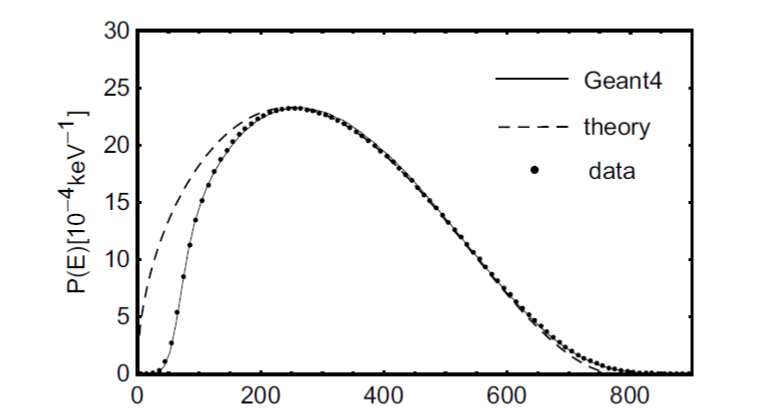
\includegraphics[width=0.78\textwidth]{NeutronBetaSpectrumUCNA.png}}
	\caption{The energy spectrum of the ultra-cold neutron measurement \cite{Hic17}}
	\label{fig:ucnabeta}
\end{figure}

There are large distortions at low energy due to back-scattering effects. 
The sample beta spectrum for this $^{20}$F measurement in figure \ref{fig:samplefit} does not show these distortions.
The systematic uncertainty quoted due to backscattering effects is $\pm 0.005$, which is larger the statistical uncertainty of this $^{20}$F measurement.
The largest systematic uncertainty in the neutron measurement was due to uncertainties in the detector calibration.
The fluorine measurement avoids this, as the gain is left as a free parameter.

Another method to get the Fierz term is by measuring $ft$ values.
From the superallowed beta decays, the result for the Fierz term is $-0.0028 \pm 0.0026$ \cite{Har17}.
It was obtained with $ft$ vaule measurements of 14 different nuclei. 
The uncertainty is the statistical uncertainty of the fit after the $ft$ values were corrected.
However, this Fierz term is sensitive to scalar couplings, and not tensor coupling like in the $^{20}$F measurement.
It had different systematic effects, and it took 14 different measurements to come up with this number.
Even with all this, the potential sensitivity to the implant technique is similar to that of 14 $ft$ value measurements.

A different measurement with sensitivity to tensor couplings was made with $^{60}$Co \cite{Wau10}.
This was a the beta asymmetry measurement, where the beta asymmetry was compared to the standard model value.
This was done with a large magnet. 
The largest uncertainty was due to the size and location of the source.
The limit on the tensor couplings was between $-0.089$ and $0.013$.
Assuming that $C_{A}' = 0$, this corresponds to a similar error bar in the Fierz term.
This uncertainty is larger than the uncertainty due to the lower beta cut effect.

In order to compare this to high energy techniques, equation \ref{eq:bgtpropor} is used \cite{Gon19}.
If the lower beta cut effect is resolved and the systematic effects described above accurate, then the total uncertainty on $b_{GT}$ is 0.0078. 
This corresponds to an uncertainty on $Re(\epsilon_{t}$ of 0.0013.
This is about twice the uncertainty from the neutral current channel at the LHC. 
Running the experiment with more statistics would help reach that uncertainty.
Then, the statistical uncertainty would be negligible, and the systematic uncertainty would be the limiting factor. 

\section{Further Refinements to Technique}
The first thing to do to improve the experiment is to run more events.
Most of the events ran for this experiment were with the PVT detector.
However, the shape of beta spectrum in that detector had an odd distortion in it.
If that could be investigated and solved, using a plastic scintillator would be an ideal candidate for this measurement.
Less of the gamma ray would be absorbed, and there would be less bremsstrahlung in the detector.

The largest systematic effect right now is the lower beta cut effect. 
A likely way to solve this issue is to adjust the level of the gamma-beta sum spectrum.
This has to be seen that it works properly with Monte Carlo.
Ultimately, the resulting offset and sum spectrum level probably are not the real, physical level.
An estimate of the systematic uncertainty due to the sum spectrum level would then have to be done, much like with the offset.
As these uncertainties depend on the slopes of the lower beta cut curves, these should get more precise as more events are built.
The slope can be seen more easily as there is the error bars get smaller.
Another method would be to compare the output of GEANT4 to that of another simulation code.
EGSnrc is being used by the collaborators from Wittenburg University. 
These results will be added to the systematic uncertainty.

In order to increase efficiency for the 1.6 MeV gamma ray, the implant detector could be more completely encased with gamma detectors.
If these gamma detectors had a higher resolution, that would mean that the signal in the implant would be much cleaner.
If that were coupled with a plastic detector, then the beta spectrum of the implant detector would be much cleaner.
This would hopefully eliminate the amount of gamma-beta sum spectrum and reduce the amount of bremstrahlung.

If these systematic effects are reduced, the next largest one has to do with the uncertainty on the measurement of $b_{WM}$.
To decrease the uncertainty of $b_{WM}$,  a new and better measurement of the width of the isobaric analogue state in $^{20}$Ne would have to be measured.
This is the parameter that dominates the uncertainty in  the calculation of $b_{WM}$ \cite{Min11}.
This would require a different type of experiment.

\section{Conclusion}
With all this in place, this measurement of the Fierz term can be one of the more precise ones, if the issue with the lower beta cut can be figured out.
Many of the systematic effects would be present in other such measurements.
The calloremetric technique could be used for other allowed Gamow-Teller transitions.
Those with higher maximum energies would need an accelerator powerful enough to implant the beam deep enough to absorb all the electron energy.
A nucleus with a lower maximum energy, such as $^{6}$He, would be more sensitive to the 1/E dependence of the Fierz term. 
This technique is a promising method for precision measurements in nuclear beta decay.

\end{document}
